%!TEX root=main.tex

\chapter{Stateful Pipeline}

% Difference between stateless/stateful stage
As defined by the OpenFlow specification, a packet entering an OpenFlow switch is processed through a pipeline comprised of a set of linked flow tables that provide matching, forwarding, and packet modification. We indicate with the term \emph{stateless stage} the processing operated by a single stateless OpenFlow's flow table. Conversely, we define as \emph{stateful stage} (Figure~\ref{f:stateful-stage}) a logical stage comprising a state table and and a flow table, and implementing our abstraction.

\begin{figure}[h]
	\centering
	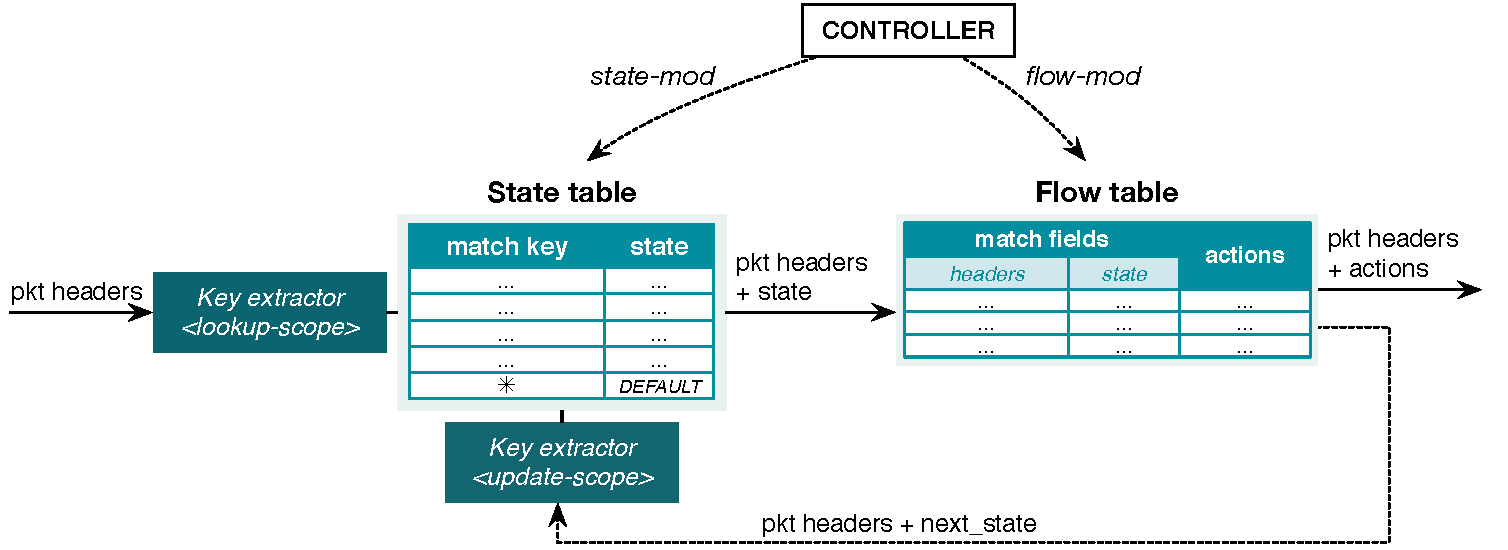
\includegraphics[width=\textwidth]{stateful-stage-arch}
	\caption{Architecture of an OpenState stateful stage}
	\label{f:stateful-stage}
\end{figure}

When a packet enters a stateful stage, it is first processed by a \emph{key extractor} which produces a string of bits representing the key to be used to match a row in the state table. The key is derived by concatenating the header fields defined in the \emph{lookup-scope}. The matched state label is appended to the packet headers as an additional header field. By exiting the state table, packet headers along with the returned state label are matched in the flow table.

The flow table is extended by adding support to a new ``state'' virtual header field to be used to match packets along with other header fields (MPLS, IP, TCP, etc.). We say this header is virtual because it is not really appended to the packet header and it is valid only for current processing trough the flow table of the stateful stage. Because state values are valid only for a specific flow (defined by the flow key), we call them ``flow states''. Finally, a new ``set-state'' action is introduced to allow the update of the state value for a given flow in a given stateful stage. The set-state action can be appended to the packet action set as any other OpenFlow action.

\comment{Carmelo}{Is it correct to say that state labels are valid only inside the stateful stage that produced them? In other words, can I match on multiple state labels provided by different stateful stages?}

\comment{Luca e Davide}{@Carmelo: It is correct! A state label can be matched only inside the stage that produced it. In a flow entry is not possible to match over multiple state fields, but it is possible to think a distributed match over multiple stages. For example, it is possible to match over a state defined in stage 1 and then, by using the metadata field to take into account the precedent match, you can process the packet in the stage 2 to match over another state. In this way you have matched over states defined in stage 1 and stage 2}

By default all the flow tables in the switch are intended as stateless stages, the controller can then enable stateful processing for one or more stages by sending a special control message to the switch and by configuring the key extractors (lookup-scope and update-scope) associated with the state table. Similarly to flow tables, new modification message called ``state-mod'' has been defined to allow the controller to configure the state entries and key extractors.

Similarly to flow states, OpenState introduces the concept of ``global states'', called also ``flags''. As suggested by the name, flags are valid globally for every packet processed by the switch. A controller can specify flags as a match field on the header packet, and it can be seen as a filtering of the flow table. A ``set-flags'' action is defined to allow the update of flags directly from the pipeline processing.
 
\comment{Carmelo}{
	Would it be useful to have ``table states''? In other words, states valid for each packet matched by a given flow table? In this case it might be useful to refer to global states as ``pipeline states'', states valid for the whole pipeline. If so, what would it be the atomicity requirements for each set-state action depending on the target (table or pipeline)?
}


%A new switch capability has been defined in order to support all the OpenState functionalities, namely flow-states and global-states. A new state modify message called \emph{state-mod} has been defined to allow the controller to configure the state entries and key extractors. Finally two new actions \textbf{set-state} and \textbf{set-flags} have been defined in order to respectively implement and configure the XFSM state transitions in the flow table and set the global states.